\subsection{Oclusión ambiental}
Al añadir sombras los objetos están mucho más integrados en la escena, pero todavía podemos conseguir un mayo grado de cohesión. En el estado actual de la escena aún hay puntos que no es convincente que reciban luz pero se encuentran totalmente iluminados. Un ejemplo son los puntos de intersección entre la esfera y el suelo. Uno esperaría que poca luz fuera capaz de alcanzar un espacio tan cóncavo, pues la propia geometría de la esfera y el suelo ocluirían la luz. Este fenómeno recibe el nombre de \textbf{oclusión ambiental}, y de nuevo gracias a los SDF nos resultará muy fácil y computacionalmente barato simularlo.\newline

Cuando se trabaja con geometría de polígonos, una de las técnicas más comunes es la oclusión ambiental del espacio de pantalla, o SSAO por sus siglas en inglés. En su versión más básica esta solución usa la información del fotograma actual para consultar por cada píxel el \textif{buffer} de profundidad o \textit{deph buffer} de los píxeles cercanos. Con esta información realiza una aproximación de las características de la geometría en ese entorno y deduce la cantidad de luz que debería poder pasar. El principal problema de esta y otras técnicas basadas en el espacio de pantalla es que al no usar la información real de la geometría, los resultados obtenidos varían según la orientación de la cámara, posición relativa de los objetos en pantalla, etc. Otro método basado en espacio de pantalla que pone de manifiesto este problema es el de los reflejos de espacio de pantalla o SSR, que suele ser usado para simular reflejos como los del agua o espejos en videojuegos. Al usar el mismo principio que SSAO, solo podrá reflejar correctamente los píxeles que estén dibujados en pantalla. Esta limitación hace que cuando un objeto ocluye a otro este no se puede reflejar correctamente y se generen reflejos erróneos como se muestra en la \autoref{fig:ssrVS}, o que si un objeto no aparece en pantalla directamente no sea reflejado, como se representa en la \autoref{fig:ssrEsquema}.

\begin{figure}[!h]
     \begin{minipage}[c]{0.49\linewidth}
        \centering
        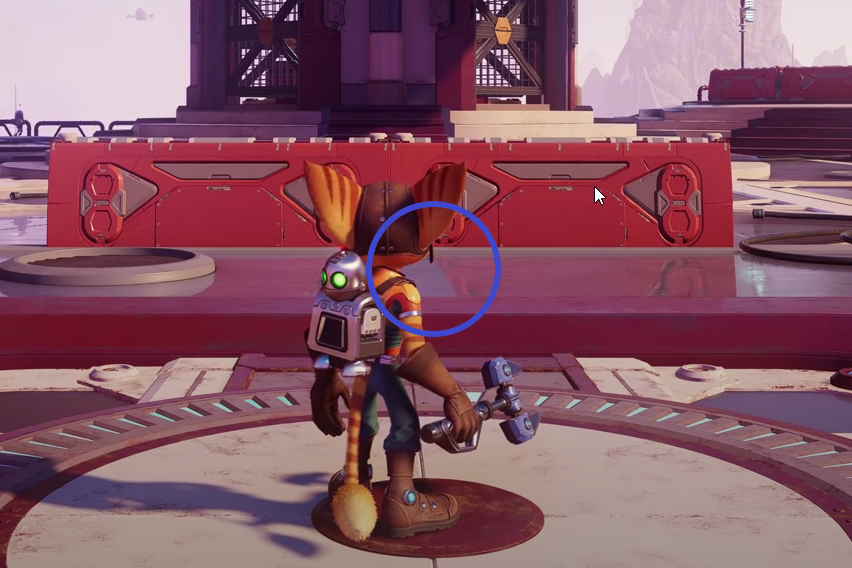
\includegraphics[width=0.98\textwidth]{Plantilla-TFG-master/img/ssr_on.png}
        \caption{SSR}
     \end{minipage}
     \begin{minipage}[c]{0.49\linewidth}
        \centering
        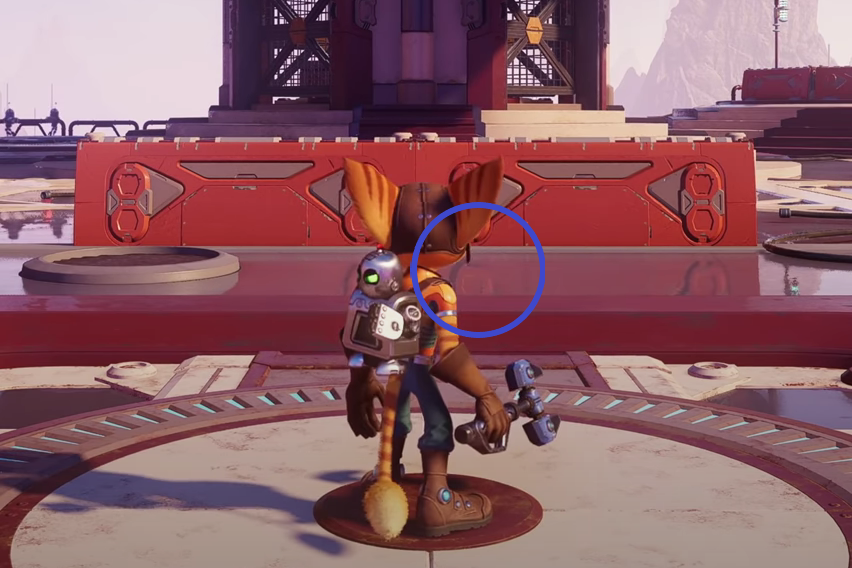
\includegraphics[width=0.98\textwidth]{Plantilla-TFG-master/img/ssr_off.png}
        \caption{\textit{Raytracing}}
     \end{minipage}
     \caption{Videojuego Ratchet \& Clank: Una dimensión aparte usando SSR y \textit{raytracing} \cite{ratchet}}
     \label{fig:ssrVS}
\end{figure}

\begin{figure}[!h]
     \begin{minipage}[c]{0.49\linewidth}
        \centering
        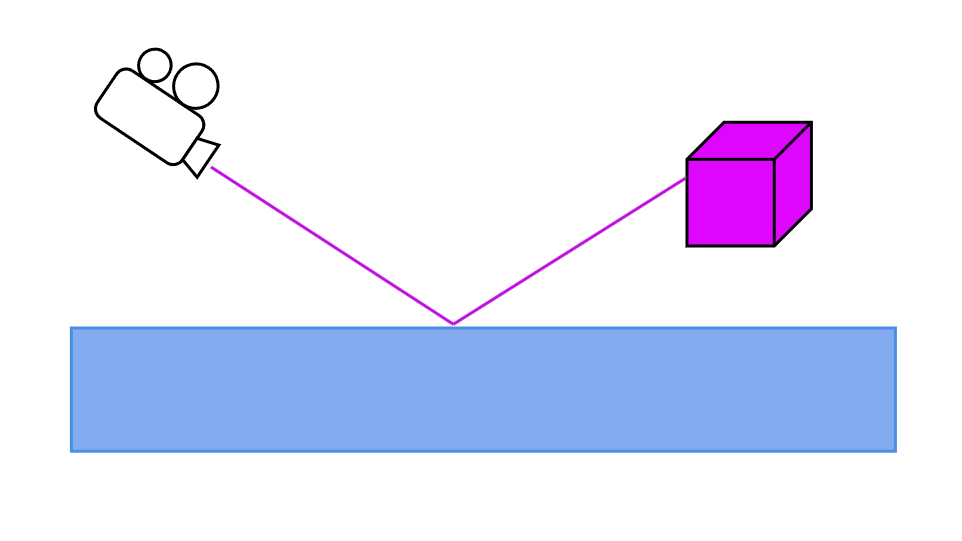
\includegraphics[width=0.9\textwidth]{Plantilla-TFG-master/img/ssr2.png}
        \caption{Reflejo detectado}
     \end{minipage}
     \begin{minipage}[c]{0.49\linewidth}
        \centering
        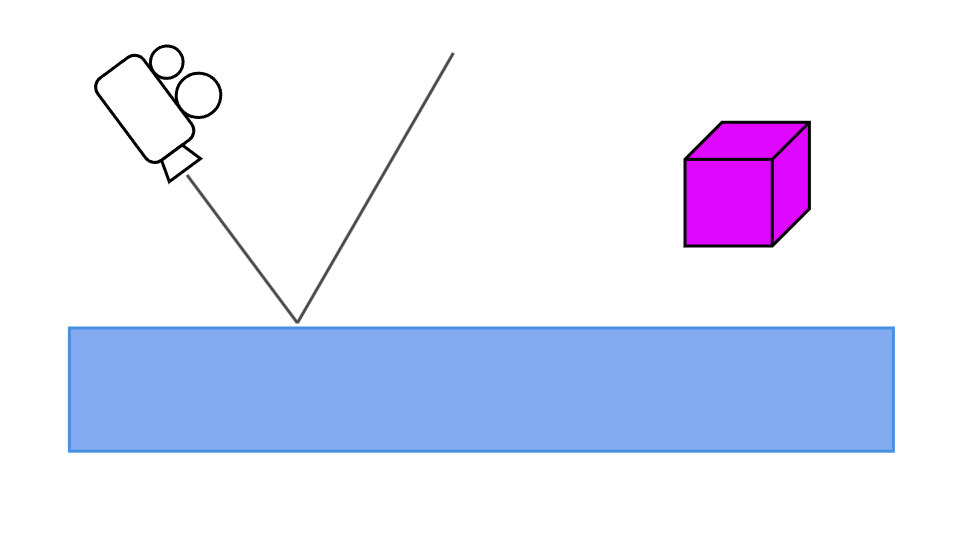
\includegraphics[width=0.9\textwidth]{Plantilla-TFG-master/img/ssr3.png}
        \caption{Reflejo no detectado}
     \end{minipage}
     \caption{Reflejos en agua con SSR}
     \label{fig:ssrEsquema}
\end{figure}

La solución a estos problemas cuando se trabaja con vértices es el uso de técnicas más avanzadas y computacionalmente costosas como el \textit{raytracing}. La buena noticia es que al estar usando SDFs nosotros podremos usar la información real de la geometría de nuestra escena. Obtendremos por tanto información más precisa, y además de forma muy barata, ya que requeriremos de muchas menos evaluaciones del SDF que el algoritmo de \textit{spheretracing}. La técnica que vamos a usar fue ideada por Alex Evans en 2006 \cite{ao}, y se conoce como \textbf{oclusión ambiental muestreada por la normal}.\newline

El método se basa en dado un punto $p\in S_{\phi}$ evaluar el SDF en varios puntos del vector normal $N_p$ a distancias $d_i$ de $p$ para obtener la información de la geometría cercana. Si en el entorno de $p$ hay geometría que le esté obstruyendo la llegada de luz, en alguna de estas evaluaciones se obtendrá un valor menor que $d_i$, mientras que de lo contrario uno esperaría que
\begin{equation*}
    \phi(p + d_i N_p) = d_i,
\end{equation*}

ya que eso significaría que el punto más cercano a $p$ de $S_{\phi}$ es el propio $p$. Así, si hacemos $M$ evaluaciones igualmente espaciadas a lo largo de $N_p$, consideraremos que el punto $p$ no está ocluido si
\begin{equation*}
    \sum_{i=1}^M \phi\Big(p + \frac{i}{M} N_p\Big) - \sum_{i=1}^M \frac{i}{M} = 0.
\end{equation*}

\begin{figure}[ht!]
    \centering
    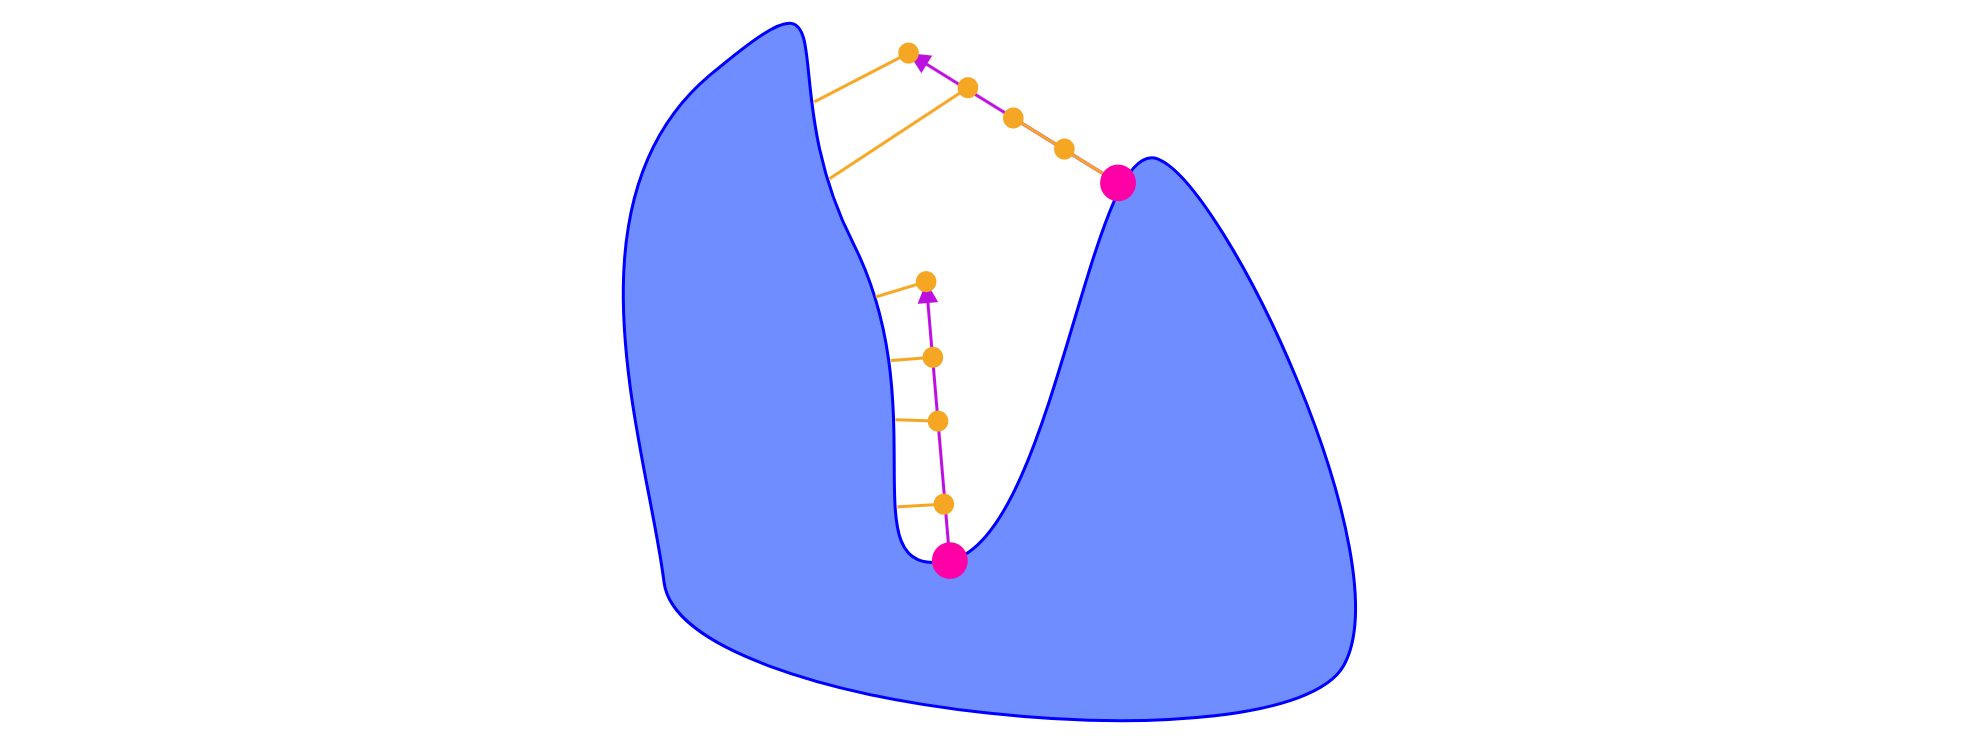
\includegraphics[width=\textwidth]{Plantilla-TFG-master/img/diagramaAO.png}
    \caption{Cálculo de oclusión ambiental muestreada por la normal}
    \label{fig:sombras4}
\end{figure}

Cuanto mayor sea este valor (no puede ser menor que $0$ por definición de SDF) menos luz será capaz de alcanzar $p$. Así, podemos representar la cantidad de luz ocluida como
\begin{equation*}
    \sum_{i=1}^M \frac{1}{2^i}\cdot \left(\frac{i}{M} - \phi\Big(p + \frac{i}{M} N_p\Big)\right)\in [0,1].
\end{equation*}

El hecho de que esté valor esté acotado en$[0,1]$ viene de que suponemos que $\Vert N_p\Vert = 1$, de forma que
\begin{equation*}
    \phi\left(p + \frac{i}{M} N_p\right) \le 1,
\end{equation*}
ya que siempre habrá algún punto a lo largo de $N_p$ que esté a una unidad o menos de distancia de $p$: él mismo. Por otro lado, hemos usado la exponencial para dar más peso sobre el resultado final a aquellos puntos más cercanos a $p$.\newline

Con esto ya podemos obtener la nueva versión del método \texttt{DibujarSuperficie} que tiene en cuenta la oclusión ambiental descrita en la \autoref{fig:dibujarAO}. En ella hemos introducido una pequeña optimización \cite{ao_opt} cambiando el índice del bucle para no tener que calcular una división en cada iteración. Otra posible optimización sería sustituir la potencia por un un flotante que fuéramos multiplicando por un factor menor que $1$ en cada iteración. Finalmente, podemos apreciar los resultados obtenidos en la \autoref{fig:resAO}, donde para valores tan pequeños de $M$ como $2$ o $4$ ya conseguimos resultados más que convincentes.

% donde hemos usado la exponencial para asegurar que $ao\in [0,1]$, que cuando no haya oclusión obtengamos $ao=1$ y que el resultado tenga un aspecto más natural. Además $k$ controlará la intensidad del efecto. Sin embargo preferiremos ganar algo de eficiencia simulando el comportamiento de la exponencial con una constante que iremos multiplicando por sí misma en cada iteración. Así, la nueva versión del método \texttt{DibujarSuperficie} será el descrito en la \autoref{fig:dibujarAO}.

\begin{figure}
    \centering
        
    \begin{algorithm}[H]
        \caption{DibujarSupercicie}
            \KwData{punto $p$, dirección del rayo $v$, distancia $\phi(p)$}
            $L \gets L_A + L_E$ \Comment{Radiancia final}
            \For{$i \in \{1,\dots, n\}$} {
    
                
                \Comment{ ··· }
                $N_p \gets CalcularNormal(p)$
                
                $sombras \gets CalcularSombras(p, l_i)$
                
                $ao \gets CalcularAO(p, N_p)$
    
                $L \gets L + S_i\cdot (f_{ra} + f_{rd} + f_{re})\cdot sombras \cdot ao$
            }
    
            \Return{$L$}
    \end{algorithm}
    
    \begin{algorithm}[H]
        \caption{CalcularAO}
            \KwData{punto $p$, vector normal $N_p$}
            \KwResult{$ao \in [0,1]$}
            $ao \gets 1$
                    
            $increment \gets \nicefrac{1}{M}$
            
            $i\gets increment$
        
            \While{$i<1$}{
                $sdf \gets \phi(p + iN_p)$
                
                $ao \gets ao - 2^{-iM}\cdot (i-sdf)$
    
                $i\gets i+increment$
            }
                
            \Return{$ao$}
    \end{algorithm}
    
    \caption{Cálculo de oclusión ambiental}
    \label{fig:dibujarAO}
\end{figure}


\begin{figure}[!h]
     \begin{minipage}[c]{0.49\linewidth}
        \centering
        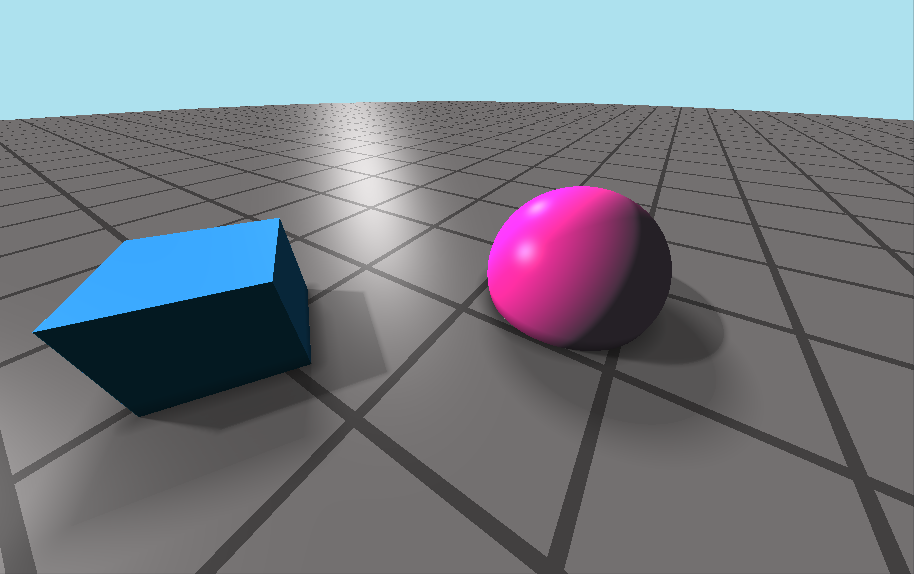
\includegraphics[width=0.98\textwidth]{Plantilla-TFG-master/img/ao2.png}
        \caption{$M=2$}
     \end{minipage}
     \begin{minipage}[c]{0.49\linewidth}
        \centering
        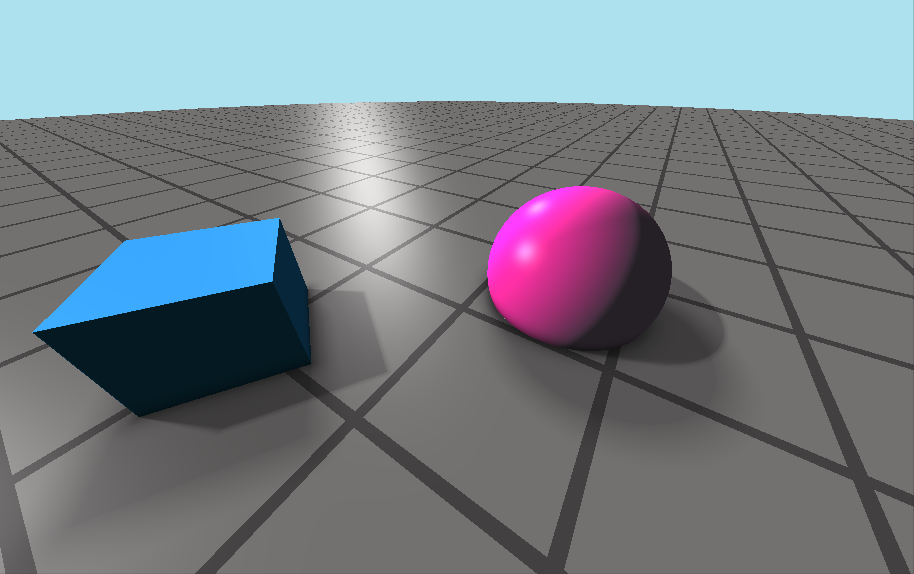
\includegraphics[width=0.98\textwidth]{Plantilla-TFG-master/img/ao4.png}
        \caption{$M=4$}
     \end{minipage}
     \caption{Resultado del cálculo de oclusión ambiental}
     \label{fig:resAO}
\end{figure}